\documentclass{beamer}

% There are many different themes available for Beamer. A comprehensive
% list with examples is given here:
% http://deic.uab.es/~iblanes/beamer_gallery/index_by_theme.html
% You can uncomment the themes below if you would like to use a different
% one:
%\usetheme{AnnArbor}
%\usetheme{Antibes}
%\usetheme{Bergen}
%\usetheme{Berkeley}
%\usetheme{Berlin}
%\usetheme{Boadilla}
%\usetheme{boxes}
%\usetheme{CambridgeUS}
%\usetheme{Copenhagen}
%\usetheme{Darmstadt}
%\usetheme{default}
%\usetheme{Frankfurt}
%\usetheme{Goettingen}
%\usetheme{Hannover}
%\usetheme{Ilmenau}
%\usetheme{JuanLesPins}
%\usetheme{Luebeck}
\usetheme{Madrid}
%\usetheme{Malmoe}
%\usetheme{Marburg}
%\usetheme{Montpellier}
%\usetheme{PaloAlto}
%\usetheme{Pittsburgh}
%\usetheme{Rochester}
%\usetheme{Singapore}
%\usetheme{Szeged}
%\usetheme{Warsaw}

\title{One Method for Convex Optimization on Square}

\author{I.~Kuruzov\inst{1} \and F.~Stonyakin\inst{1, 2}}
% - Give the names in the same order as the appear in the paper.
% - Use the \inst{?} command only if the authors have different
%   affiliation.

\institute[MIPT] % (optional, but mostly needed)
{
  \inst{1}%
Moscow Institute of Physics and Technology
  \and
  \inst{2}%
V.I.Vernadsky Crimean Federal University}
% - Use the \inst command only if there are several affiliations.
% - Keep it simple, no one is interested in your street address.

\date{COG, 2019}
% - Either use conference name or its abbreviation.
% - Not really informative to the audience, more for people (including
%   yourself) who are reading the slides online

\subject{Theoretical Computer Science}
% This is only inserted into the PDF information catalog. Can be left
% out. 

% If you have a file called "university-logo-filename.xxx", where xxx
% is a graphic format that can be processed by latex or pdflatex,
% resp., then you can add a logo as follows:

% \pgfdeclareimage[height=0.5cm]{university-logo}{university-logo-filename}
% \logo{\pgfuseimage{university-logo}}

% Delete this, if you do not want the table of contents to pop up at
% the beginning of each subsection:
\AtBeginSubsection[]
{
  \begin{frame}<beamer>{Outline}
    \tableofcontents[currentsection,currentsubsection]
  \end{frame}
}

% Let's get started
\DeclareMathOperator{\sign}{sign}
\begin{document}

\begin{frame}
  \titlepage
\end{frame}


\begin{frame}{Method Description}
Task:
$$\min_{(x,y)}\left\{f(x,y)|(x,y) \in Q\right\},$$
where $f$ is a convex function, $Q = [a,b]\times[c, d]\in \mathbb{R}^2$.

\begin{block}{One iteration}
\begin{itemize}
\item{Find minimum with accuracy $\delta$ on central horizontal segment in square and calculate gradient at this point\pause}
\item{Choose rectangle which anti-gradient looks in\pause}
\item{Analogically for vertical segment in the rectangle}
\end{itemize}
\end{block}
\end{frame}

\begin{frame}{Plan}
  \tableofcontents
  % You might wish to add the option [pausesections]
\end{frame}

% Section and subsections will appear in the presentation overview
% and table of contents.

\section{Strategy for segment accuracy}


\begin{frame}{Strategies}{True Gradient}
Let $f$ be convex and has $L$-Lipschitz continuous gradient.
    $$\sign f'_y(x_0) = \sign f'_y(x_{current})$$
    
For this it is sufficient:
    $$|f'_y(x_0) - f'_y(x_{current})| \leq |f'_y(x_0)|$$
	\pause
  $$\boxed{\delta < \frac{|f'_y(x_{0})|}{L}}$$
\end{frame}

\begin{frame}{Strategies}{Current Gradient}
    $$\sign f'_y(x_0) = \sign f'_y(x_{current})$$
    
For this it is sufficient:
    $$|f'_y(x_0) - f'_y(x_{current})| \leq |f'_y(x_{current})|$$
	\pause
  $$\boxed{\delta < \frac{|f'_y(x_{current})|}{L}}$$
\end{frame}

\begin{frame}{Strategies}{Small Gradient}
But what can we do when norm of gradient is small?

\pause
\begin{block}{Small Gradient}
Let $f$ be convex and has $L$-Lipschitz continuous gradient. Then for accuracy on function $\epsilon$ following condition in point $\textbf{x}$ is sufficient:

$$\|\nabla f(\textbf{x})\|\leq \frac{\epsilon}{a\sqrt{2}}, $$
where $a$ is size of current square.
\end{block}
\end{frame}

\section{Convergence}

\begin{frame}{Convergence}
Function $f$ is convex. Size of square $Q$ is equal to $a$. One takes a center of a current square as approximate  solution.
\begin{block}{Estimate through Lipschitz function constant}
Let function $f$ be $L_f$-Lipschitz continuous. Then for accuracy $\epsilon$ on function it is sufficient:
\begin{equation}\label{NI1}N = \left\lceil\log_2\frac{L_fa}{\sqrt{2}\epsilon}\right\rceil.\end{equation}
\end{block}
\pause
\begin{block}{Estimate through Lipschitz gradient constant}
Let function $f$ have $L_g$-Lipschitz continuous gradient. Moreover, point with zero derivative is  \textbf{internal point}. Then for accuracy $\epsilon$ on function it is sufficient:
\begin{equation}\label{NI3}N = \left\lceil\frac{1}{2}\log_2\frac{L_ga^2}{4\epsilon}\right\rceil.\end{equation}
\end{block}
\end{frame}

\section{Convergence}

\begin{frame}{Convergence}
If following inequallity is met
$$\frac{2L_f^2}{L_g} \geq \epsilon$$
then the estimate through $L_g$ is better than through $L_f$.
\end{frame}

\section{Tests}

\begin{frame}{Experiments}{Test Functions}

\begin{itemize}
\item{Quadratic Function

$$f(x,y) = (Ax+By)^2+Cy^2 + Dx+Ey$$
$$(x^*, y^*)\in Q$$
$$L_f = \max\limits_{(x,y) \in Q}\|\nabla f(x, y)\|$$
$$L_g = \max |\lambda\left(H(f)\right)|$$
}
\end{itemize}
\end{frame}

\begin{frame}{Experiments}{Iterations Number}


Theoretical Iteration Number through function constant equals 40

Theoretical Iteration Number through gradient constant equals 20
\pause
\begin{figure}[h!]
\center{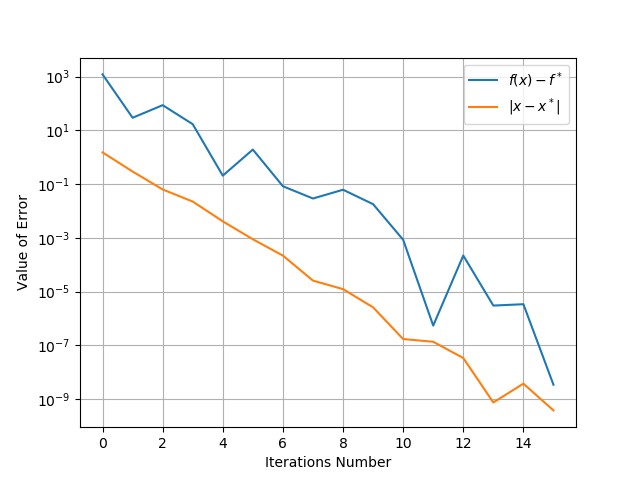
\includegraphics[scale=0.3]{In_point.png}}
\label{fig:image}
\end{figure}
\end{frame}

\begin{frame}{Experiments}{Iterations Number}

$$f(x,y) = (x+y)^2+x^2, Q = [1,2]^2,\,(x^*, y^*) = (1,1)$$

Theoretical Iteration Number through function constant 30

Theoretical Iteration Number through gradient constant 14

\pause

\begin{figure}[h!]
\center{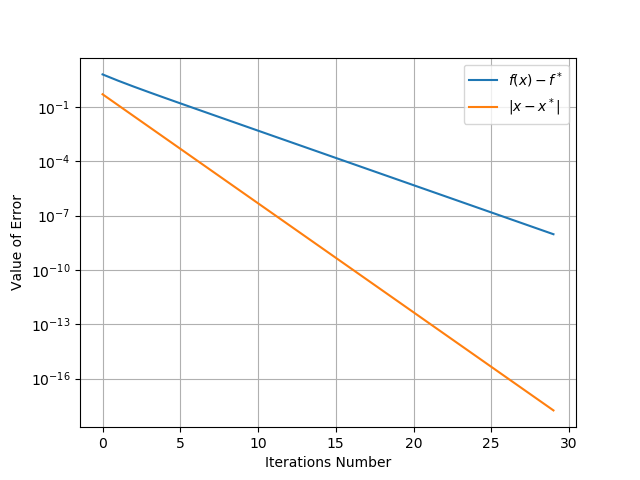
\includegraphics[scale=0.3]{Out_point.png}}
\label{fig:image}
\end{figure}
\end{frame}

\begin{frame}{Experiments}{Comparison Of Methods}

\begin{figure}[h!]
\center{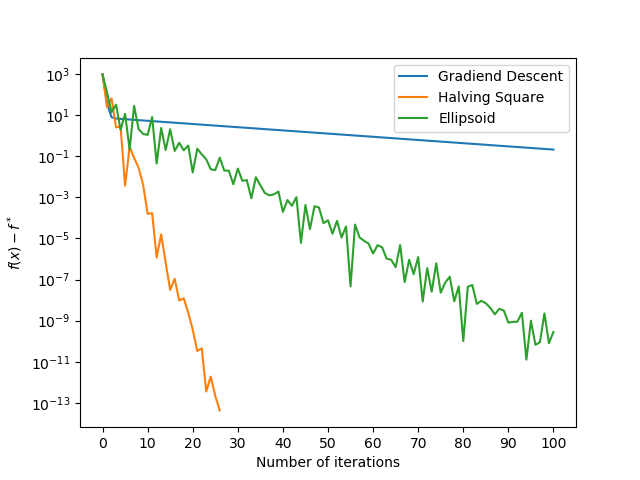
\includegraphics[scale=0.4]{GD_HS_EL.png}}
\label{fig:image}
\end{figure}

\end{frame}

\begin{frame}{Experiments}{Comparison Of Methods}

\begin{block}{Work time}
Gradiend Descent 4.5 ms

Halving Square 20.9 ms

Ellipsoid 28.3 ms
\end{block}
\end{frame}

\section*{Summary}

\begin{frame}{Summary}
  \begin{itemize}
  \item
    Strategy for solution on segment
  \item
    Convergence Results
  \item
    Experiments for this method
        \begin{itemize}
    \item
      Iterations number
    \item
      Comparison with different methods
    \end{itemize}
  \end{itemize}
\end{frame}

\end{document}


